\chapter{Gauss's Law}
\label{chapter:gauss}

\section{Flux}
\textbf{Flux} is an important concept in many disciplines in physics. The
flux of a vector quantity $\bm X$ is the amount of that quantity flowing
through a surface. In integral form:
\begin{equation}
  \Phi=\int\bm X\cdot\dl{\bm A}
  %\quad\text{or}\quad
  %\Phi=\int(\bm X\cdot\hat{\bm n})\dl A
\end{equation}

Suppose we want to find the volumetric flow rate of water through the mouth
of a hose.

Now we note that when water exits the mouth of the hose, the velocity vector
does not necessarily have to be perpendicular to the surface. Therefore, we
separate the velocity vector into the component perpendicular to the surface
$\bm v_\perp$, and the component parallel to the surface $\bm v_\parallel$. It
should be apparent that $\bm v_\parallel$ does not actually flow \emph{out} of
the hose, leaving only the perpendicular component:
\begin{equation*}
  \Phi_\text{volume}=\bm v_\perp A=(\bm v\cdot\hat{\bm n})A
\end{equation*}
where $\hat{\bm n}$ is the outward normal direction of the surface. For
convenience, we would incorporate this direction into the area $A$, turning it
into a vector $\bm A$:
\begin{equation*}
  \Phi_\text{volume}=\bm v\cdot\bm A
\end{equation*}
This equation would apply if the velocity across the mouth of the hose is
uniform. But the water velocities out of the mouth of the hose is never
uniform, i.e.\ $\bm v$ is a function of position\footnote{And possibly a
function of time as well} $\bm v=\bm v(x,y,z)$, so instead of multiplying the
velocity vector by the area $\bm A$, we must instead \emph{integrate} over the
cross sectional area of the hose to compute the volumetric flow rate:
\begin{equation*}
  \Phi_\text{volume}=\int_{\mathcal S}\bm v\cdot\dl{\bm A}
\end{equation*}
As before, the direction of $\dl{\bm A}$ is the outward normal from the surface.
This volumetric flow rate can also be called the \emph{velocity flux}. If we
are interested in the \emph{mass flow rate} instead, we can replace the
velocity vector field with momentum, i.e.\ multiplying by the fluid density:
\begin{equation*}
  \Phi_\text{mass}=\int_{\mathcal S}(\rho\bm v)\cdot\dl{\bm A}
\end{equation*}
The mass flow rate is also called the \emph{momentum flux}. Flux through a
surface can be of something physical, like the flow of water out of the mouth
of a hose, but it can also be \emph{any} vector field $\bm X=\bm X(x,y,z)$ that
passes through a surface $\mathcal S$. In this chapter, we are interested in
the flux of  the electric field, called the \textbf{electric flux}:
\begin{equation}
  \Phi_E=\int_\mathcal{S}\bm E\cdot\dl{\bm A}
\end{equation}


%The direction of the infinitesimal area $\dl{\bm A}$ is \textbf{outward normal}
%to the surface.
%\begin{center}
%  \pic{.3}{electrostatics2/eflux}
%\end{center}
%$\Phi$
%something abstract, like electric field (which is what we are interested
%in). We can compute a flux as long as there is a vector field i.e.\
%In the case of \textbf{electric flux}, the quantity
%$\bm X$ is just the electric field:





\section{Gauss's Law}
\textbf{Gauss's law for electricity} tells us that for a closed surface
$\mathcal S$ (think of the surface of a balloon), the total electric flux is
given by:
\begin{equation}
  \boxed{
    \Phi_E=\oint_{\mathcal S}\bm E\cdot\dl{\bm A}
    =\frac{Q_\text{encl}}{\epsilon_0}
  }
\end{equation}    
where $Q_\text{encl}$ is the charge enclosed by the surface, and
$\epsilon_0=\SI{8.85e-12}{C^2/N.m^2}$ is the permittivity of free space.
That closed surface is called a \textbf{Gaussian surface}. Gauss's law is
derived from Coulomb's law.



%\section{Closed Surfaces}
%A \textbf{closed surface} is one that does not have a boundary, like the
%sphere, toroid, and cube on the left.
%\begin{figure}[ht]
%  \centering
%  \pic{.5}{electrostatics2/800px-SurfacesWithAndWithoutBoundary}
%\end{figure} 


Since Gauss's law is a \emph{fundamental} equation, it should apply to
\emph{any} arbitrary-shaped Gaussian surface around \emph{any} arbitrary
distribution of charges, like those shown in Fig.~\ref{fig:2-gaussians}. In the
present example, two arbitrary Gaussian surfaces ($S_1$ and $S_2$) enclose an
arbitrarily-shaped charge $Q_\text{encl}$. The electric field at $\mathcal S_1$
is stronger, but the electric flux is integrated over a smaller Gaussian
surface, while the electric field at $\mathcal S_2$ is weaker than
$\mathcal S_1$ because the Gaussian surface is farther away from the charge,
but the electric flux is integrated over a much larger surface.
\begin{figure}[ht]
  \centering
  \begin{tikzpicture}[scale=.5]
    \node (0) at (-4.25, 0.75) {};
    \node (1) at (-2.25, 1) {};
    \node (2) at (-4.5, -0.25) {};
    \node (3) at (-2.5, -0.25) {};
    \node (4) at (1.25, 1.75) {};
    \node (5) at (-0.75, 3) {};
    \node (6) at (-5.5, 3) {};
    \node (7) at (-7.5, 0.25) {};
    \node (8) at (-5.25, -2.5) {};
    \node (9) at (0, -1) {};
    \node (10) at (4.25, 4.25) {};
    \node (11) at (-2.5, 5.25) {};
    \node (12) at (-9.75, 4.75) {};
    \node (13) at (-10.75, -1) {};
    \node (15) at (-3, -5) {};
    \node (16) at (4.5, -1) {};

    \draw[very thick,pattern=north east lines] (1.center)
    to[in=45, out=-180, looseness=1.5] (0.center)
    to[in=135, out=-135, looseness=0.75] (2.center)
    to[in=165, out=-60, looseness=0.75] (3.center)
    to[in=0, out=-15, looseness=1.25] (1.center);
  
    \shade[ball color=orange,opacity=.7] (5.center)
    to[in=15,out=-150] (6.center)
    to[in=105,out=-165] (7.center)
    to[in=180,out=-75] (8.center)
    to[in=165,out=0,looseness=1.25] (9.center)
    to[in=-75,out=0] (4.center)
    to[in=30,out=105,looseness=.75] (5.center);

    \draw[thick,orange] (5.center)
    to[in=15,out=-150] (6.center)
    to[in=105,out=-165] (7.center)
    to[in=180,out=-75] (8.center)
    to[in=165,out=0,looseness=1.25] (9.center)
    to[in=-75,out=0] (4.center)
    to[in=30,out=105,looseness=.75] (5.center);
    
    \begin{scope}[vector,orange]
      \draw (-5,2.5)--+(-.5,1.7);
      \draw (-4,2.5)--+(-.3,2);
      \draw (-3,2.5)--+(.1,2) node[right]{$\bm E$};
      \draw (-2,2.2)--+(.4,1.8);
      \draw (-1,2.35)--+(.7,1.8);
    \end{scope}
    
    \shade[ball color=violet,opacity=.2] (10.center)
    to[in=0,out=150,looseness=1.50] (11.center)
    to[in=30,out=-180] (12.center)
    to[in=90,out=-150,looseness=1.5] (13.center)
    to[in=150,out=-90,looseness=1.25] (15.center)
    to[in=-90,out=-30,looseness=.75] (16.center)
    to[in=-30,out=90,looseness=.75]  (10.center);

    \draw[thick,violet] (10.center)
    to[in=0,out=150,looseness=1.50] (11.center)
    to[in=30,out=-180] (12.center)
    to[in=90,out=-150,looseness=1.5] (13.center)
    to[in=150,out=-90,looseness=1.25] (15.center)
    to[in=-90,out=-30,looseness=.75] (16.center)
    to[in=-30,out=90,looseness=.75]  (10.center);

    \begin{scope}[vector,violet]
      \draw (-9.75,4.4)--+(-.5,.6);
      \draw (-8,5.1)--+(-.4,.8);
      \draw (-6,5.3)--+(-.3,.8) node[right]{$\bm E$};
      \draw (-4,5.2)--+(-.2,.7);
      \draw (-2,5.1)--+(.1,.8);
      \draw (0,5.2)--+(.2,.6);
      \draw (2,5.2)--+(.4,.5);
    \end{scope}
    \draw[thick] (-3.3,.5) to[out=270,in=90] +(2,-2)
    node[below]{$Q_\text{encl}$};
    \node[right,violet] at (4.3,4.3) {$\mathcal S_2$};
    \node[right,orange] at (1.3,1.8) {$\mathcal S_1$};
  \end{tikzpicture}
  \caption{Two different Gaussian surfaces over the same enclosed charge}
  \label{fig:2-gaussians}
\end{figure}
However, regardless of the shape and size of the Gaussian surfaces, the total
electric flux $\Phi_E$ out of $\mathcal S_1$ and $\mathcal S_2$ are the same:
\begin{equation*}
  \Phi_E=
  {\color{orange}\oint_{\mathcal S_1}\bm E\cdot\dl{\bm A}}=
  {\color{violet}\oint_{\mathcal S_2}\bm E\cdot\dl{\bm A}}=
  \frac{Q_\text{encl}}{\epsilon_0}
\end{equation*}

It must be pointed out that using the Gauss's law in practice is not always
straightforward: while the right-hand side of the equation
($q_\text{encl}/\epsilon_0$) is a simple expression, the integral on the left
hand side ($\oint\bm E\cdot\dl{\bm A}$) can be extremely difficult and
impractical to do. Therefore, in the practical use of Gauss's law, we seek
configurations with high degrees of symmetry, where the integral can turn in to
an algebraic expression.


\subsection{Electric Field from a Point Charge}
We can use Gauss's law to find the magnitude of the electric field near a
point charge $q$. We place a spherical Gaussian surface of radius $r$,
with the centre of the Gaussian sphere at the point charge, as shown in
Fig.~\ref{fig:pt-charge-gaussian}. In this case, the point charge is positive,
and the electric field is radially outward, in the $+\hat{\bm r}$-direction
(i.e.\ $E$ is only a function of $r$).
\begin{figure}[ht]
  \centering
  \begin{tikzpicture}[scale=1.2]
    \foreach \x in {0,15,...,359}{
      \draw[orange,vector,rotate=\x] (0,0)--(0,1);
      \draw[orange,very thick,rotate=\x] (0,0)--(0,2.3);
    }
    \shade[ball color=orange] circle (.15);
    \node[orange,right] at (2,0) (E) {$\bm E$};
    
    \draw[violet] circle (1.5);
    \shade[ball color=violet,opacity=.5] circle (1.5);
    \draw[axes,violet] (0,1.5)--(0,2.2) node[above]{$\hat{\bm n}$};
  \end{tikzpicture}
  \caption{Spherical Gaussian surface around a point charge}
  \label{fig:pt-charge-gaussian}
\end{figure}
Likewise, the outward normal direction $\hat{\bm n}$ of the Gaussian surface is
also along $+\hat{\bm r}$. By symmetry, the integral on the left hand side
reduces to a multiple:
\begin{equation*}
  \Phi_E=\oint_{\mathcal S}\bm E\cdot\dl{\bm A}=EA=\frac q{\epsilon_0}
\end{equation*}
Since the surface area of a sphere is $A=4\pi r^2$, we find that the magnitude
of the electric field to be:
\begin{equation*}
  E=\frac q{\epsilon_0A}=\frac1{4\pi\epsilon_0}\frac q{r^2}=\frac{kq}{r^2}
\end{equation*}
Of course, we recover the expression that we have already defined in
Eq.~\ref{eq:pt-charge-E}.




\subsection{Electric Field from a Uniformly-Charged Spherical Shell}
Consider a uniformly-charged spherical thin shell with radius $R$ and a total
charge of $Q$, as shown in Fig.~\ref{fig:spherical-charged-shell}.
\begin{figure}[ht]
  \centering
  \begin{tikzpicture}
    \draw[thick,fill=red!70!black] circle (1.5);
    \draw[thick,fill=white] circle (1.45);
    \draw[axes,rotate=60] (0,0)--(1.5,0) node[above]{$R$};

    \foreach \x in {0,15,...,359}{
      \draw[orange,vector,rotate=\x] (0,1.5)--+(0,1);
      \draw[orange,very thick,rotate=\x] (0,1.5)--+(0,1.5);
    }
    
    \shade[ball color=red,opacity=.7] circle (1.5);
    
    \draw[axes] (0,0)--(1,0) node[right]{$r_i$};
    \draw[dashed,thick] circle (1);
    
    \draw[axes,rotate=-50] (0,0)--(2.25,0) node[below]{$r_0$};
    \draw[dashed,thick] circle (2.25);
  \end{tikzpicture}
  \caption{Gaussian surfaces inside and outside a spherical charge.}
  \label{fig:spherical-charged-shell}
\end{figure}
The thickness $t$ of the shell is negligible (i.e.\ $t\ll R$). In this case, we
are interested in the electric field inside ($r_i<R$) and outside ($r_o>R$) the
sphere. To analyis the electric field, we contruct two spherical Gaussian
surfaces concentric with the sphere, one inside and one outside the sphere.

\textbf{Inside the shell ($r_i<R$):} There is no enclosed charge, therefore
the electric field must be zero:
\begin{equation*}
  \oint_{\mathcal S}\bm E\cdot\dl{\bm A}=\frac{q_\text{encl}}{\epsilon_0}=0
  \quad\quad\longrightarrow\quad\quad E=0
\end{equation*}
\textbf{Outside the shell ($r_o>R$):} The entire spherical charge is inside the
Gaussian surface, therefore enclosed charge is $Q$. By symmetry, the
magnitude of the electric field must be the same throughout the Gaussian
surface, and with a direction in in the outwardly radial ($+\hat{\bm r}$)
direction, which is also the outward normal direction of the Gaussian surface.
Like the point charge, integration can be avoid:
\begin{equation}
  \oint_{\mathcal S}\bm E\cdot\dl{\bm A}=\frac Q{\epsilon_0}
  \quad\quad\longrightarrow\quad\quad E=\frac Q{\epsilon_0A}
  =\frac1{4\pi\epsilon_0}\left[\frac Q{r^2}\right]
\end{equation}
Electric field outside a spherical shell is the same equation as the point
charge.

Fig.~\ref{fig:E-spherical-shell} shows the electric field strength $|\bm E|$ as
a function of the distance $r$ from the centre of the shell.
\begin{figure}[ht]
  \centering
  \begin{tikzpicture}
    \draw[axes] (0,0)--(0,3) node[above]{$|\bm E|$};
    \draw[axes] (0,0)--(5.5,0) node[right]{$r$};
    \draw[dashed] (1,0)--(1,2) node[pos=0,below]{$R$}
    --(0,2) node[left]{$\dfrac1{4\pi\epsilon_0}\dfrac Q{R^2}$};
    \draw[function,smooth,domain=1:5] plot(\x,{2/\x});
    \draw[function] (0,0)--(1,0);
    \draw[function,fill=white] (1,0) circle (.06);
    \fill[red!80!black] (1,2) circle (.06);
  \end{tikzpicture}
  \caption{Electric field strength inside and outside of the uniformly-charge
    sphere}
  \label{fig:E-spherical-shell}
\end{figure}
This graph may be familiar, because the graph for the gravitational field
strength inside a uniform shell (Fig.~\ref{fig:spherical-shells}) is exactly
the same. This shows that Gauss's law can also be used to compute gravitational
fields of symmetrical masses. To adapt the law for gravity, we replace the
constant $\epsilon_0$ with $-4\pi G$.\footnote{The negative sign is necessary
because for a positive charge, the electric field lines are outwardly away
from the charge, whereas for masses, the gravitational field lines are inward,
toward the masses.}



%\section{Worksheet Examples}
%  Follow the worksheet for these examples:
%  \begin{itemize}
\subsection{Electric Fields from a Uniformly-Charged Sphere}
For a slightly more difficult example, consider a uniformly-charged sphere
with radius $R$ and a total charge of $Q$, as shown in
Fig.~\ref{fig:uniform-spherical-charge}. The charge is evenly spread over the
entire volume of the sphere.
\begin{figure}[ht]
  \centering
  \begin{tikzpicture}
    \foreach \x in {0,15,...,359}{
      \draw[orange,vector,rotate=\x] (0,1.5)--+(0,1);
      \draw[orange,very thick,rotate=\x] (0,1.5)--+(0,1.5);
    }
    \draw[thick,red] circle (1.5);
    \shade[ball color=red,opacity=.6] circle (1.5);
   
    \draw[axes] (0,0)--(1,0) node[right]{$r_i$};
    \draw[dashed,thick] circle (1);

    \draw[axes,rotate=-50] (0,0)--(2.4,0) node[below]{$r_o$};
    \draw[dashed,thick] circle (2.4);
  \end{tikzpicture}
  \caption{Gaussian surfaces inside and outside a spherical charge.}
  \label{fig:uniform-spherical-charge}
\end{figure}
Again, we are interested in the electric field inside ($r_i<R$) and outside
($r_o>R$) the sphere. To analyis the electric field, we contruct two spherical
Gaussian surfaces concentric with the sphere, one inside and one outside the
sphere.

\textbf{Inside the sphere ($r_i<R$):} We must first calculate the charge
enclosed by the Gaussian surface. Since the sphere is uniformly charged, the
charge density is
\begin{equation*}
  \rho=\frac QV=\frac{3Q}{4\pi R^3}
\end{equation*}
and the enclosed charge is therefore
\begin{equation*}
  q_\text{encl}(r)=\rho V(r)=\frac{3Q}{4\pi R^3}\left(\frac43\pi r^3\right)
  =\left(\frac{r^3}{R^3}\right)Q
\end{equation*}
By symmetry, electric field strength must be constant throughout the
Gaussian surface, therefore integration can be avoided. 
%There is no enclosed charge, therefore
%the electric field must be zero:
\begin{equation*}
  \oint_{\mathcal S}\bm E\cdot\dl{\bm A}=\frac{q_\text{encl}}{\epsilon_0}
  \quad\quad\longrightarrow\quad\quad EA=\frac Q{\epsilon_0}\frac{r^3}{R^3}
\end{equation*}
Solving for $E$, we find that it is linear with the distance from the centre
of the sphere:
\begin{equation*}
  E=\frac Q{\epsilon_0A}\frac{r^3}{R^3}
  =\frac Q{\epsilon_0(A\pi r^2)}\frac{r^3}{R^3}
  =\frac Q{4\pi\epsilon_0}\left[\frac r{R^3}\right]
\end{equation*}
\textbf{Outside the sphere ($r_o>R$):} The entire spherical charge is inside the
Gaussian surface, therefore enclosed charge is $Q$. By symmetry, the
magnitude of the electric field must be the same throughout the Gaussian
surface, and with a direction in in the outwardly radial ($+\hat{\bm r}$)
direction, which is also the outward normal direction of the Gaussian surface.
Like the point charge, integration can be avoid:
\begin{equation}
  \oint_{\mathcal S}\bm E\cdot\dl{\bm A}=\frac Q{\epsilon_0}
  \quad\quad\longrightarrow\quad\quad E=\frac Q{\epsilon_0A}
  =\frac1{4\pi\epsilon_0}\left[\frac Q{r^2}\right]
\end{equation}
Electric field outside a sphere is the same equation as the point charge.

\begin{figure}[ht]
  \centering
  \begin{tikzpicture}
    \draw[axes] (0,0)--(0,3) node[above]{$|\bm E|$};
    \draw[axes] (0,0)--(5.5,0) node[right]{$r$};
    \draw[thick,dashed] (1,0)--(1,2) node[pos=0,below]{$R$}--(0,2)
    node[left]{$\dfrac1{4\pi\epsilon_0}\dfrac Q{R^2}$};
    \draw[function,domain=1:5] plot(\x,{2/\x});
    \draw[function] (0,0)--(1,2);
  \end{tikzpicture}
  \caption{Electric field strength inside and outside a uniform-charged sphere
    of radius $R$.}
  \label{fig:E-sphere}
\end{figure}
The electric field strength is zero at the centre inside the sphere, and
the increases linearly to the surface $r=R$, then drops off as $1/r^2$ outside
the sphere.

\fcolorbox{black}{pink!10}{
  \begin{minipage}{.97\linewidth}
    \textbf{Common question: Does it matter if the sphere is a conductor or
      not?} Yes it does.
  \end{minipage}
}

%\subsection{Charged sphere with variable charge density}



\subsection{Infinitely-long charge rod with uniform density}
Gauss's law can be used to find the electric fields inside and outside an
infinitely-long charged rod of radius $R$ with uniform charge density,
as shown in Fig.~\ref{fig:charged-rod}. In this
example, since the rod is infinitely long, the total charge would be infinite,
it would be easier to describe the charge by its charge density $\rho$.
\begin{figure}[ht]
  \centering
  \begin{subfigure}{.6\linewidth}
    \centering
    \begin{tikzpicture}[scale=.6]
      \draw[thick,dashed,violet,fill=violet!30,opacity=.2] (0,2.8)--(8,2.8)
      arc (90:270:1.4 and 2.8)--(0,-2.8) arc(270:90:1.4 and 2.8);

      \draw[thick,fill=lightgray] ellipse (1 and 2);

      \draw[thick,dashed,magenta,fill=magenta!30,opacity=.3] (0,1)--(8,1)
      arc (90:270:.5 and 1)--(0,-1) arc(270:90:.5 and 1);
      \draw[thick,dashed,magenta,fill=magenta!50,opacity=.3] (0,1)--(8,1)
      arc (90:-90:.5 and 1)--(0,-1) arc(-90:90:.5 and 1);
      
      \draw[thick,fill=gray] (0,2)--(8,2) arc (90:-90:1 and 2)--(0,-2)
      arc (-90:90:1 and 2);

      \draw[thick] (-5,0)--(0,0);
      \draw[thick] (9,0)--(11,0);
      \draw[thick,dashed] (-5,2)--(11,2);
      \draw[thick,dashed] (-5,-2)--(11,-2);
      \draw[thick,dashed,violet] ellipse (1.4 and 2.8);
      \draw[thick,dashed,violet,fill=violet!50,opacity=.2] (0,2.8)--(8,2.8)
      arc (90:-90:1.4 and 2.8)--(0,-2.8) arc(-90:90:1.4 and 2.8);
      \foreach \x in {0,...,8}{
        \draw[vector,orange!50] (\x,2.8)--(\x,4.1);
        \draw[vector,orange!50] (\x,-2.8)--(\x,-4);
      }
      \draw[violet] (7.5,-2.8)--(6,-5) node[left]{Gaussian surface};
    \end{tikzpicture}
  \end{subfigure}
  \begin{subfigure}{.25\linewidth}
    \centering
    \begin{tikzpicture}[scale=.6]
      \draw[thick,fill=lightgray] circle (2);
      \fill circle (.05);

      \foreach \x in {0,30,...,359}{
        \draw[orange,vector,rotate=\x] (0,0)--(0,1.8);
        \draw[orange,very thick,rotate=\x] (0,0)--(0,2);
        \draw[orange!50,vector,rotate=\x] (0,2)--(0,4);
      }
      \draw[axes,rotate=-45] (0,0)--(2,0) node[right]{$R$};
      \draw[thick,dashed,magenta] circle (1);
      \draw[thick,dashed,violet] circle (2.8);
      \begin{scope}[rotate=-110,violet]
        \draw[axes] (0,0)--(2.8,0) node[right]{$r_o$};
        \draw (0,0)--(5,0) node[right]{Gaussian surface};
      \end{scope}
    \end{tikzpicture}
  \end{subfigure}
  \caption{Infinitely-Long charged rod with uniform charge density}
  \label{fig:charged-rod}
\end{figure}

\textbf{Inside the rod:} By symmetry, the electric field must only be in the
radial direction: radially outward if the rod is positively charged, and
radially inward if negative. Here we assume that the rod is positively charged.
We then contruct a cylindrical Gaussian surface with radius $r_i<R$ and length
$L$ that aligns with the axis of the rod. Since the electric field is radial,
there is no flux through the ends of the Gaussian surface, only through the
side. The total charge enclosed by the Gaussian surface is:
\begin{equation*}
  q_\text{encl}=\rho V_\text{encl}=\rho(\pi r_i^2L)
\end{equation*}
Substituting this into Gauss's law, and simplifying the terms:
\begin{equation*}
  \oint_{\mathcal S}\bm E\cdot\dl{\bm A}=EA=\frac{q_\text{encl}}{\epsilon_0}
  \quad\longrightarrow\quad
  E=\frac{q_\text{encl}}{\epsilon_0A}
  =\frac{\rho\pi r_i^2L}{\epsilon_0(2\pi r_iL)}
  =\left[\frac\rho{2\epsilon_0}\right]r_i
\end{equation*}
Inside the rod, electric field strength scales linearly with the distance from
the axis of the rod.

\textbf{Outside the rod:} The symmetry, the electric field outside the rod
must also be entirely in the radial direction. Again, we construct a
cylindrical Gaussian surface of radius $r_o>R$ and length $L$ as before. The
enclosed charge is therefore:
\begin{equation*}
  q_\text{encl}=\rho\pi R^2L
\end{equation*}
Substituting this into Gauss's law:
\begin{equation*}
  \oint_{\mathcal S}\bm E\cdot\dl{\bm A}=EA=\frac{q_\text{encl}}{\epsilon_0}
  \quad\longrightarrow\quad
  E=\frac{q_\text{encl}}{\epsilon_0A}
  =\frac{\rho\pi R^2L}{\epsilon_0(2\pi r_oL)}
  =\left[\frac{\rho R^2}{2\epsilon_0}\right]\frac1{r_o}
\end{equation*}
Outside the rod, electric field strength is inversely proprotional to the
distance from axis of the rod.



\subsection{Electric Field Near an Infinite Plane of Charge}
\begin{figure}[ht]
  \centering
  \pic{.45}{electrostatics2/elec_gauss_figure9}
\end{figure}

\begin{itemize}
\item Charge density (charge per unit area) $\sigma$
\item By symmetry, $\bm E$ must be perpendicular to the plane
\item Our Gaussian surface is a cylinder shown in the left with an area
  $A$; the height of the cylinder is unimportant
\item Nothing ``flows out'' of the side of the cylinder, only at the ends
\item The total flux is $\Phi_E=E(2A)$
\item The enclosed charge is $Q_\text{encl}=\sigma A$
\end{itemize}
  
Gauss's law simplifies to:
\begin{equation}
  \oint_{\mathcal S}\bm E\cdot\dl{\bm A}=\frac{q_\text{encl}}{\epsilon_0}
  \;\rightarrow\;
  E(2A)=\frac{\sigma A}{\epsilon_0}
\end{equation}
Solving for $E$, we get:
\begin{equation}
  \boxed{
    E=\frac\sigma{2\epsilon_0}
  }
\end{equation}
Electric field $E$ is constant away from the plane charge, and is independent
of the distance from the plnate.
%\begin{itemize}
%\item $E$ is a constant
%\item Independent of distance from the plane
%\item Both sides of the plane are the same
%\end{itemize}
  




\subsection{Electric Field Between Parallel Charged Plates}
\begin{figure}[ht]
  \centering
  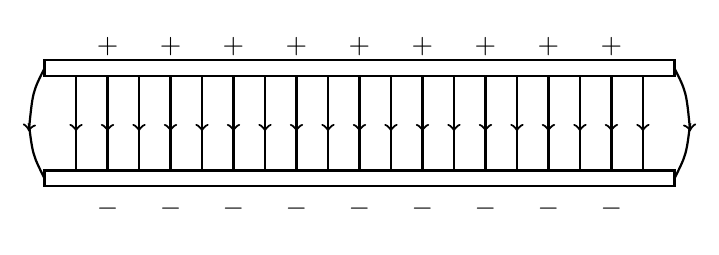
\begin{tikzpicture}[thick]
    \draw rectangle (8,.2);
    \draw (0,1.4) rectangle (8,1.6);
    \foreach \x in {.4,.8,1.2,...,7.6}{
      \draw[->] (\x,1.4)--(\x,.7);
      \draw (\x,1.4)--(\x,.2);
    }
    \foreach \x in {.8,1.6,2.4,...,7.2}{
      \node at (\x,1.78) {$\bm{+}$};
      \node at (\x,-.28) {$\bm{-}$};
    }
    
    \draw[->] (0,1.5) ..controls(-.15,1.2).. (-.2,.7);
    \draw (-.2,.8) ..controls(-.15,.4).. (0,.1);
    
    \draw[->] (8,1.5) ..controls(8.15,1.2).. (8.2,.7);
    \draw (8.2,.8) ..controls(8.15,.4).. (8,.1);
  \end{tikzpicture}
\end{figure}

\begin{itemize}
\item Two plates, each producing an electric field pointing in
  the same direction
\item The total electric field is twice the value of \emph{one} infinite
  plane, pointing from the positively charged plate toward the negatively
  charged plate
  \begin{equation}
    \boxed{E=\frac\sigma{\epsilon_0}}
  \end{equation}
\item $\bm E$ outside the plates is very low (close to zero), except for
  fringe effects at the edges of the plates
\end{itemize}
Recall that electric field ($\bm E$) is the negative gradient of electric
potential difference ($V$):
\begin{equation*}
  \bm E=-\diffp Vr\hat{\bm r}
\end{equation*}
This relationship holds regardless of the charge configuration. In the case of
two parallel plates, the electric field is uniform, and the relationship
simplifies to:
\begin{equation}
  \boxed{E=\frac{\Delta V}d\quad\text{(parallel plates)}}
\end{equation}
where $\Delta V$ is the electric potential difference (voltage) across the
plates, and $d$ is the distance between the plates.
%\begin{figure}[ht]
%  \centering
%  \begin{subfigure}{.48\linewidth}
%    \centering
%    \begin{tikzpicture}[scale=.45]
%      \draw[thick,violet] rectangle +(15,.3);
%      \draw[thick,orange] (0,2) rectangle +(15,.3);
%      \foreach \x in {.5,1.5,...,14.5}{
%        \node[violet] at (\x,.15) {\scriptsize $-$};
%        \node[orange] at (\x,2.15) {\scriptsize $+$};
%        
%        \draw[vector,orange] (\x,2.3)--+(0,1.2);
%        \draw[vector,orange] (\x,2)--+(0,-1.2);
%        \draw[very thick,orange] (\x,2.3)--+(0,2.5);
%        \draw[very thick,orange] (\x,2)--+(0,-4);
%
%%      \draw[vector,violet] (\x+.2,1.5)--+(0,-1.2);
%%      \draw[vector,violet] (\x+.2,-1.2)--+(0,1.2);
%%      \draw[very thick,violet] (\x+.2,.3)--+(0,4);
%        %      \draw[very thick,violet] (\x+.2,0)--+(0,-2.5);
%      }
%    \end{tikzpicture}
%  \end{subfigure}
%  \begin{subfigure}{.48\linewidth}
%    \centering
%    \begin{tikzpicture}[scale=.45]
%      \draw[thick] rectangle +(15,.3);
%      \draw[thick] (0,2) rectangle +(15,.3);
%      \foreach \x in {.5,1.5,...,14.5}{
%        \node at (\x,.15) {\scriptsize $-$};
%        \node at (\x,2.15) {\scriptsize $+$};
%        
%        \draw[vector,orange] (\x,2)--(\x,1);
%        \draw[very thick,orange] (\x,2)--(\x,.3);
%      }
%    \end{tikzpicture}
%  \end{subfigure}
%\end{figure}
